\documentclass[11pt,aspectratio=1610,xcolor=dvipsnames]{beamer}

\usetheme[
    background=light,
    numbering=fraction,
    block=fill,
    progressbar=frametitle
]{metropolis}

\usepackage[style=authortitle-ibid,backend=biber]{biblatex}
\addbibresource{refs.bib}
\setbeamerfont{footnote}{size=\scriptsize}

\usepackage{physics}
\usepackage{bbm}
\usepackage{booktabs}
\usepackage[most,skins,theorems]{tcolorbox}
\tcbset{variables/.style={colback=yellow!20,colframe=yellow}}
\usepackage{tikz}
\usetikzlibrary{arrows}
% \colorlet{LightLavender}{Lavender!40!}
\newtcolorbox{prob}{colback=red!5!white,colframe=red!75!black}
\usefonttheme[onlymath]{serif}
\usepackage{quantikz}

\newcommand{\R}{\mathbb{R}}
\newcommand{\U}[1]{\mathsf{U}(#1)}
\newcommand{\defeq}{\stackrel{\text{\tiny def}}{=}}

\titlegraphic{
\includegraphics[width=0.3\textwidth]{unitary_fund_logo.png}}

\title{Quantum Wednesday}
\subtitle{\href{https://arxiv.org/abs/2201.10672}{\texttt{arXiv:2201.10672}}}
\date{Nov 16, 2022}
\author{Nate Stemen}


\begin{document}

\maketitle

\begin{frame}{Today's Paper}
	\begin{figure}[h]
		\centering
		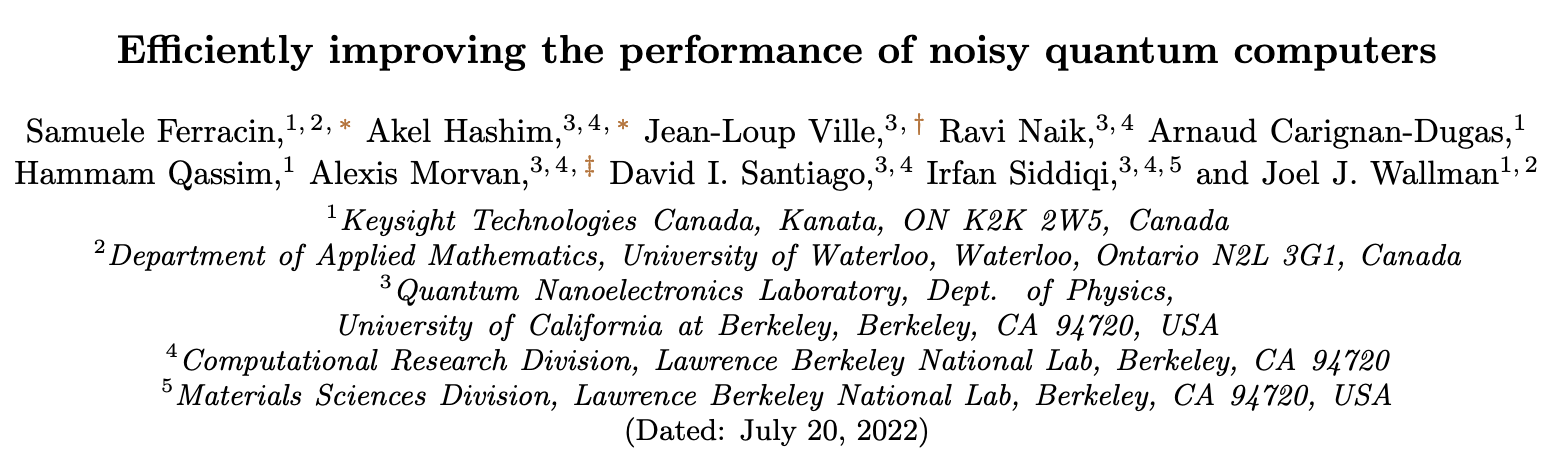
\includegraphics[width=\textwidth]{paper.png}
	\end{figure}
	\begin{center}
		\url{https://arxiv.org/abs/2201.10672}
	\end{center}
	\note[item]{
		authors, who's who
		\item paper came on the arxiv earlier this year
		\item presents ideas very similar to some that we know and use in mitiq
		\item it's both a theory and experimental paper and it's short and sweet. it also has the strange power of making the reader sick. both times i've had a serious read through this paper i've gotten sick
	}
\end{frame}

\begin{frame}{Main Ideas}
	% \begin{columns}
	% 	\begin{column}{0.6\textwidth}
	\begin{itemize}
		\item Noiseless Output Extrapolation (NOX)
		\item Pauli Error Cancellation (PEC)
	\end{itemize}
	% \end{column}
	\uncover<2>{
		% \begin{column}{0.45\textwidth}
		\begin{tcolorbox}[title=Question,halign title=center,halign=center,colback=orange!20, colframe=orange!80]
			\Large
			How are these different from Zero-Noise Extrapolation (ZNE) and Probabilistic Error Cancellation (PEC)?
		\end{tcolorbox}
		% \end{column}
	}
	% \end{columns}
\end{frame}

\setbeamercovered{transparent}
\begin{frame}{Cycles}
	\begin{columns}
		\begin{column}{0.6\textwidth}
			\begin{center}
				\begin{quantikz}[slice all]
					& \gate{} & \ctrl{1}  & \gate{} & \targ{}   & \gate{} & \targ{}   & \gate{} & \ctrl{1} & \qw \\
					& \qw     & \targ{}   & \gate{} & \ctrl{-1} & \qw     & \ctrl{-1} & \gate{} & \targ{}  & \qw \\
					& \qw     & \targ{}   & \gate{} & \qw       & \gate{} & \targ{}   & \qw     & \ctrl{1} & \qw \\
					& \gate{} & \ctrl{-1} & \gate{} & \qw       & \qw     & \ctrl{-1} & \qw     & \targ{}  & \qw
				\end{quantikz}
			\end{center}
			\uncover<2->{
				\begin{align}
					\mathcal{C} & = \mathcal{E}_{m + 1} \mathcal{H}_m \mathcal{E}_m \cdots \mathcal{E}_2 \mathcal{H}_1 \mathcal{E}_1 \\
					            & \eqqcolon \mathcal{E}_{m + 1}\qty(\mathop{\circ}\limits_{j = 1}^m \mathcal{H}_j \mathcal{E}_j)
				\end{align}
			}
		\end{column}
		\begin{column}{0.4\textwidth}
			\uncover<2->{
				\begin{tcolorbox}[variables]
					% - Calligraphic letters denote CPTP maps

					- $\mathcal{E}_i$: single qubit cycles

					- $\mathcal{H}_i$: Clifford two-qubit cycles
				\end{tcolorbox}
			}
		\end{column}
	\end{columns}
\end{frame}

\begin{frame}{Cycle Error Reconstruction\footcite{cer} (CER)}
	\begin{figure}
		\centering
		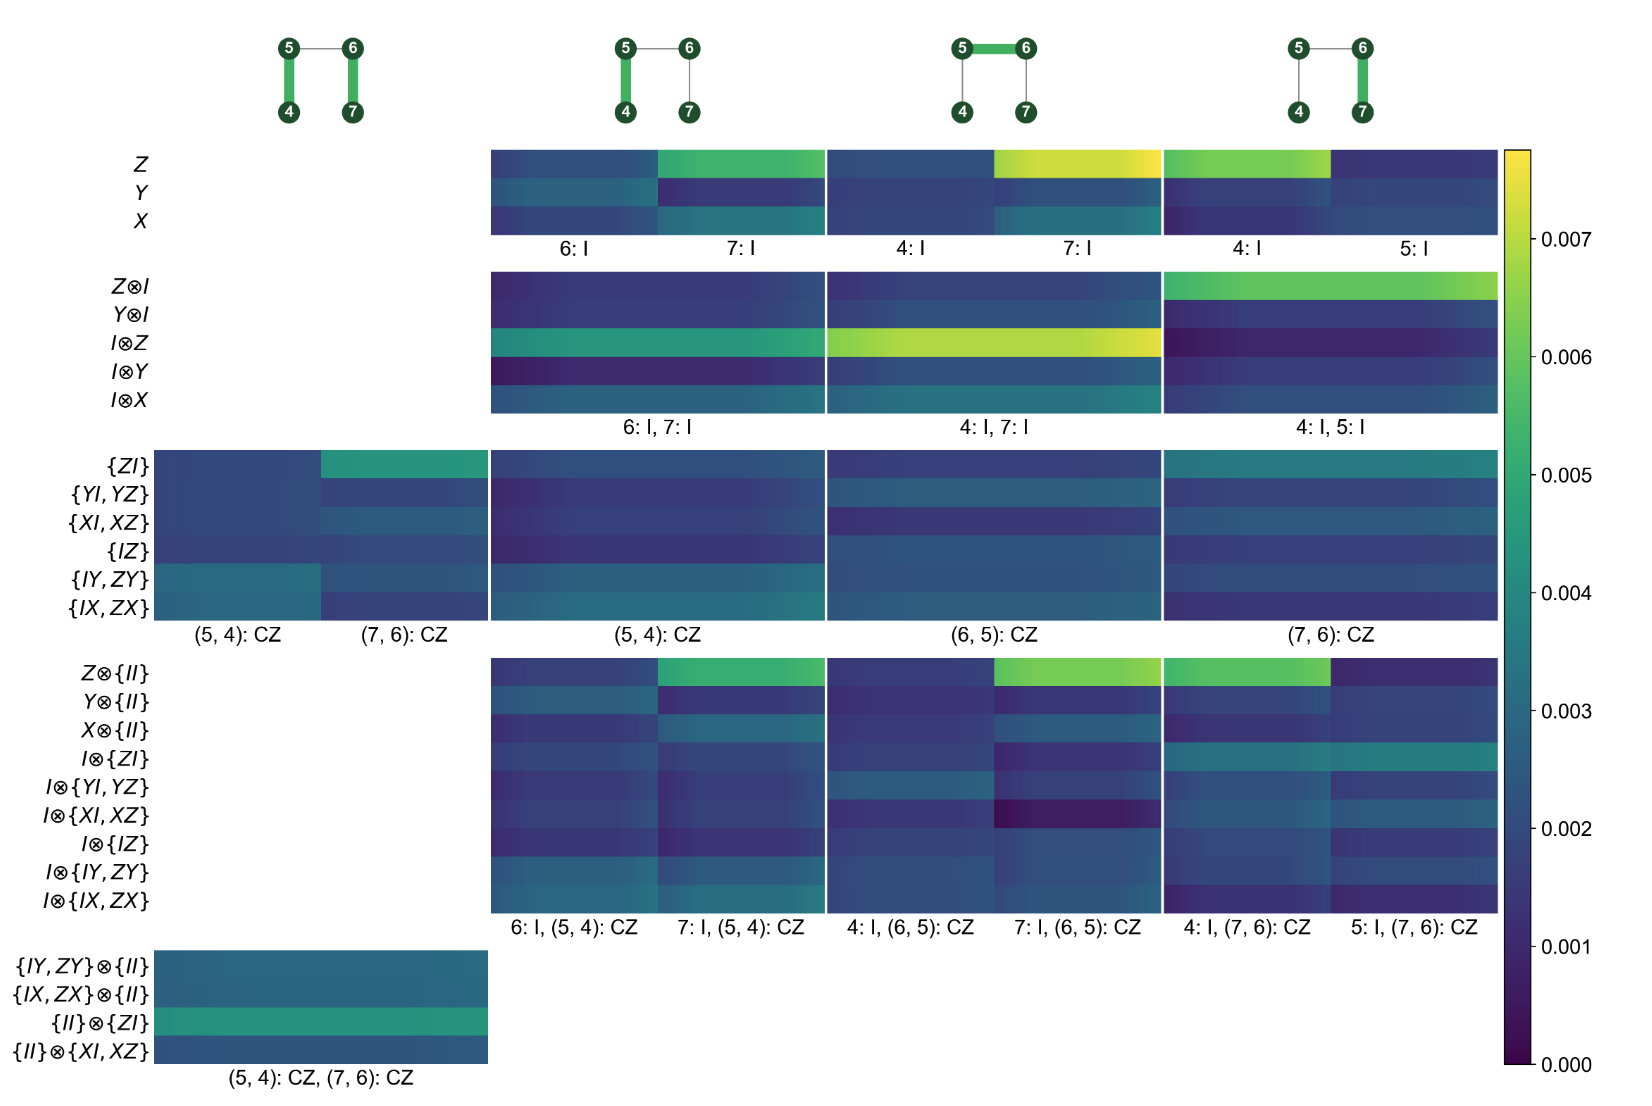
\includegraphics[width=0.75\textwidth]{cerdata.png}
	\end{figure}
\end{frame}

\begin{frame}{Setup}
	\uncover<+->{\textbf{Assumptions}:}
	\begin{enumerate}[<+->]
		\item Noise is Markovian and time stationary ($\mathcal{D}_\mathcal{U}\,\mathcal{U}$).
		\item $\mathcal{D}_\mathcal{U} = \mathcal{D}$ when $\mathcal{U}$ consists solely of single qubit gates ($\mathcal{D}_{\mathcal{E}_i}\mathcal{E}_i = \mathcal{D}\mathcal{E}_i$ for all $i$).
	\end{enumerate}
	\uncover<+->{
		Noise processes $\mathcal{D}_\mathcal{U}$ taken to be a Pauli channels by Randomized Compiling.\footcite{randcomp}
	}
	\uncover<+->{
		\begin{columns}
			\begin{column}{0.5\textwidth}
				\begin{equation*}
					\mathcal{D}_\mathcal{U}(\rho) = \sum_{k = 0}^{4^n - 1} \epsilon_k^{(\mathcal{U})} \mathcal{P}_k(\rho)
				\end{equation*}
			\end{column}
			\begin{column}{0.5\textwidth}
				\begin{tcolorbox}[ams align*, variables]
					\mathcal{P}_k & \in \qty{\mathcal{I}, \mathcal{X}, \mathcal{Y}, \mathcal{Z}}^{\otimes n} \\
					\epsilon_k^{(\mathcal{U})} & \text{: Pauli error rates}
				\end{tcolorbox}
			\end{column}
		\end{columns}
	}
	\note{In practice, not all $4^n - 1$ error rates are studied, only $K$-body errors, which significantly reduces overhead, and is realistic to make a cutoff.

		the authors note that nonmarkovianity does happen, however
	}
\end{frame}

\begin{frame}{Noiseless Output Extrapolation}
	\begin{itemize}[<+->]
		\item Need a way to scale the noise: $\mathcal{D}_{\mathcal{H}_i} \mathcal{H}_i \to \mathcal{D}_{\mathcal{H}_i}^\alpha \mathcal{H}_i$
		\item ZNE uses pulse stretching, or unitary folding\footnote{This is referred to as "identity insertion" in the paper.}: $\mathcal{H}_i(\mathcal{H}_i\mathcal{H}_i^{-1})^\alpha$
		      \begin{enumerate}
			      \item $\mathcal{H}_i$ and $\mathcal{H}_i^{-1}$ have identical noise models
			      \item $\mathcal{D}_{\mathcal{H}_i}\mathcal{H}_i = \mathcal{H}_i\mathcal{D}_{\mathcal{H}_i}$
		      \end{enumerate}
		\item CER can detect when these assumptions apply
		\item Otherwise, scale noise from single cycle: $\mathcal{C}'_{j, \alpha} = \mathcal{E}_{m + 1}\mathcal{D}_{\mathcal{H}_m}\mathcal{H}_m\mathcal{E}_m \cdots \qty(\mathcal{D}_{\mathcal{H}_j})^\alpha \mathcal{H}_j \cdots \mathcal{D}_{\mathcal{H}_1}\mathcal{H}_1\mathcal{E}_1$
	\end{itemize}
	\uncover<+->{
		\begin{equation}
			\expval{O} \approx E_\text{NOX}(O) \coloneqq E_\text{noisy}(O) + \sum_{j = 1}^m \frac{E_\text{noisy}(O) - E_{j,\alpha}(O)}{\alpha - 1}
		\end{equation}
	}

	% \begin{tcolorbox}
	% 	Uses noise characterization data to inform noise scaling
	% \end{tcolorbox}
	\note{
		unitary folding can lead to very long circuits in some instances which, if drift is bad, can lead to wrong results
	}
\end{frame}

\begin{frame}{Pauli Error Cancellation}
	\begin{columns}
		\begin{column}{0.6\textwidth}
			\begin{itemize}
				\item Like Prob. EC, start with quasiprobability distribution: $C_\text{tot}\sum\limits_{i = 1}^L s_i q_i \tr(O\widetilde{\mathcal{U}}_i(\rho_\text{in})) = \tr\!\qty\big[O\mathcal{U}(\rho_\text{in})] + \delta$
				      % \item $\mathcal{E}_{m + 1}\qty(\mathop{\circ}\limits_{j = 1}^m \mathcal{P}_j \mathcal{H}_j \mathcal{E}_j)$
			\end{itemize}
		\end{column}
		\begin{column}{0.45\textwidth}
			\begin{tcolorbox}[variables]
				- $\widetilde{\mathcal{U}}_i$: implementable operations

				% - $\mathcal{P}_j \in \qty{\mathcal{I}, \mathcal{X}, \mathcal{Y}, \mathcal{Z}}^{\otimes n}$

				- $s_k = \pm 1$ depending on number of Pauli cycles

				- $r_k$ results from PEC circuits
			\end{tcolorbox}
		\end{column}
	\end{columns}
	\uncover<2->{
		\begin{align}
			C_\text{tot} & = \prod_{j = 1}^m\frac{1}{\qty\big(\epsilon_0^{(\mathcal{H}_j)})^2 - \sum_{k = 1}^{4^n - 1}\qty\big(\epsilon_k^{(\mathcal{H}_j)})^2} \\
			\expval{O}   & \approx E_\text{PEC}(O) = C_\text{tot}\sum\limits_{k = 1}^N \frac{s_k r_k}{N}
		\end{align}
	}

	\note{PEC circuits are run through randomized compiling}
\end{frame}


\begin{frame}{Summary}
	\begin{figure}[h]
		\centering
		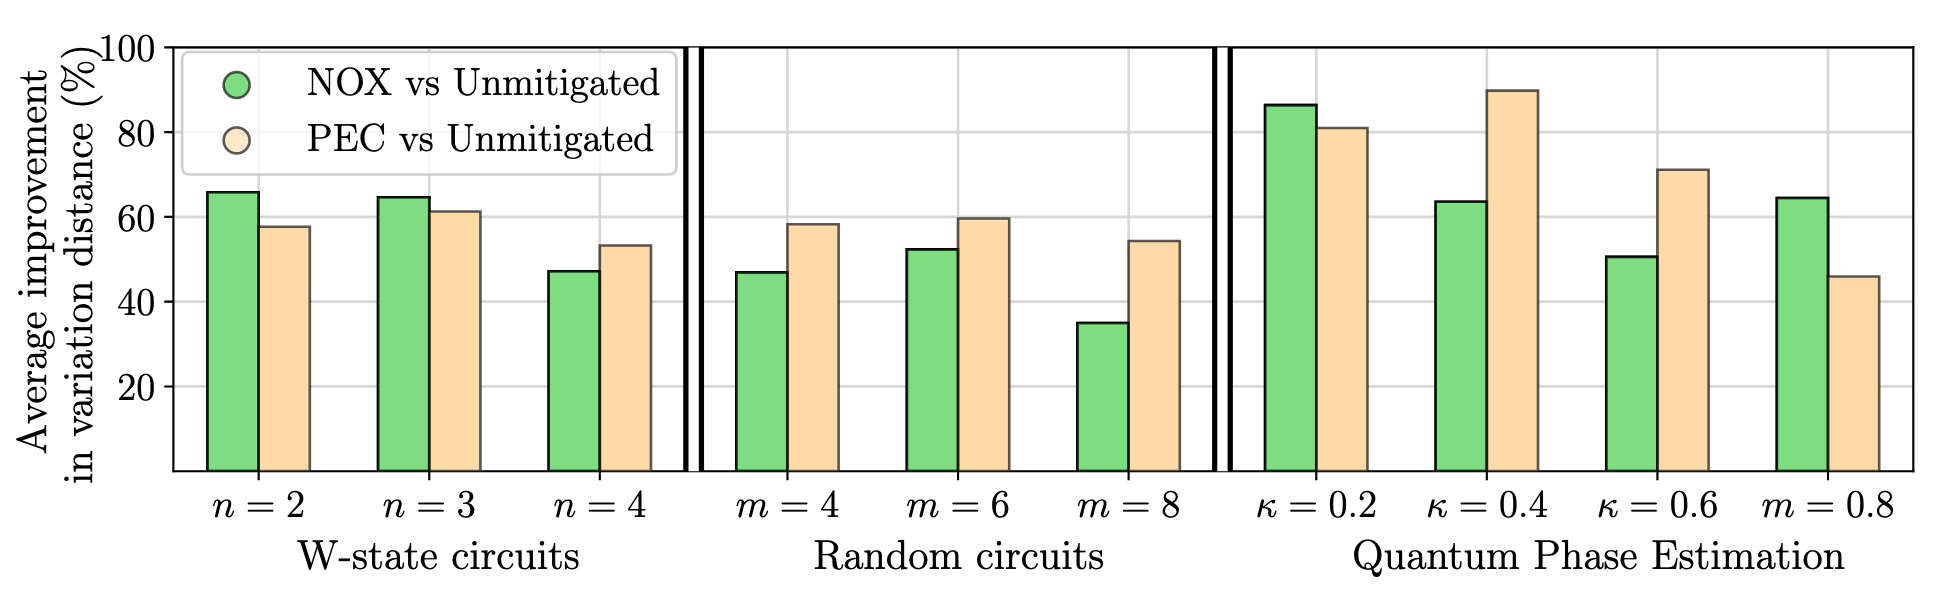
\includegraphics[width=0.9\textwidth]{results.png}
	\end{figure}
	\begin{columns}<2->
		\begin{column}{0.7\textwidth}
			\begin{table}[h]
				\centering\begin{tabular}{r | c  c  c}
					        & PEC                                             & NOX                                               & Unmit.                  \\ \toprule
					Runtime & $\frac{1}{(1-n\varepsilon)^{2m}}$               & $m^3$                                             & $1$                     \\
					Bias    & $\order{mn^2\varepsilon^2} + \delta_\text{rec}$ & $\order{m^2n^2\varepsilon^2} + \delta_\text{rec}$ & $\order{mn\varepsilon}$
				\end{tabular}
			\end{table}
		\end{column}
		\begin{column}{0.35\textwidth}
			\begin{tcolorbox}[variables]
				- $m$ circuit depth

				- $n\varepsilon$ cycle error rate

				- $n$ number of qubits

				- $\delta_\text{rec}$ accuracy of noise reconstruction
			\end{tcolorbox}
		\end{column}
	\end{columns}
	\note{
		REM used in addition to these techniques

		they did see a failure of these techniques with larger circuits. EM is not magic, it does not apply everywhere, especially on very large circuits where many body errors can occur
	}
\end{frame}

\begin{frame}{References}
	\nocite{*}
	\printbibliography[heading=none]
\end{frame}

\begin{frame}[standout]
	Thank you!
\end{frame}

\end{document}
